\chapter{CodeIgniter framework}

\assignment{MH: at number of places in this chapter I note that things are
not properly explained and introduced\ldots but maybe in fact the there are
some unnecessary details here which could also be omitted (e.g. routing,
autoloading, etc. (Not sure though -- depends on how much we want build on
top of these also in the following chapters)}

CodeIgniter is an Application Development Framework -- a toolkit -- for people who build web sites using PHP  \cite{codeigniter}. One of its goals is to provide exceptional performance of web applications along with minimum complexity and fast development. CodeIgniter was born from ExpressionEngine \cite{codeigniter} in 2006 and since then, it increasingly gained popularity among PHP developers. In 2008 CodeIginiter became industry leader in an enviroment saturated with PHP frameworks \cite{codeigniter} and in 2014 CodeIgniter v 2.2 was released. 

In this chapter, we will present a short overview of CodeIgniter request and response processing with explanation of MVC and HMVC design patterns for purposes of Chapter \ref{sec:courses}, Chapter \ref{sec:teamprojects}, respectively Chapter \ref{sec:other}.

\section{Request and response flow}

\begin{figure}[h]
    \centering
    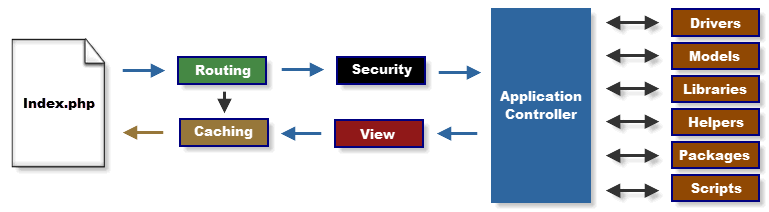
\includegraphics[width=0.85\textwidth]{images/codeigniter.png}
    \caption{CodeIgniter request flow}
    \label{codeigniter_flow}
\end{figure}


To understand how CodeIgniter works, we have to look at processing of HTTP requests. CodeIgniter uses Apache2  module \texttt{mod\_rewrite}. This ensures, that all requests are handled to \texttt{index.php} script as seen on image \ref{codeigniter_flow}. Purpose of this script is to load configuration of the whole application and other classes. This file is provided by CodeIgniter framework and should not be changed (only for configuration purposes).

Before any of the user written code is loaded, the HTTP request and any user submitted data is filtered for security. To process HTTP request, router must decide the correct operation over it. Each module of application must have it's own routes defined as follows:

\begin{lstlisting}[basicstyle=\small,caption={CodeIgniter routing}]
$route[course/(:num)] = "courses/$1";
\end{lstlisting}

The application takes list of all routes and applies the one of which regexp pattern matches the request URL. After this operation, proper controller (to be defined in the next subsection) is selected, instanciated and method \texttt{run()} of this controller is run.

\section{Model-View-Controller}
For software to be usefult, it has to interact with something. This could be another computer or process, or the interaction could be with people. So, there are interfaces. In modern applications, more effort often goes into development of usable interface than in other tasks. On the other side, our software needs to acces and store its data and perform operations on them.

Purpose of this section is, at first, to explain Model-View-Controller (MVC) design pattern, which is a simple and widespread way for solving this problem. We also aim to explain how MVC is implemented in CodeIgniter with examples.

In an Object Oriented Programming (OOP) programmers often run into problems with application complexity and maintanance of code. As application becomes larger and more robust, it is ofter harder to add or modify existing features. Modifying of complex classes and unclear implementation can cause a lot of software bugs. On the other way, design patterns aim to provide reusable soulutions of common problems in software engineering and reduce this complexity by splitting functionality into specific classes with a single purpose. One of the most important desing patterns is Model View-Controller, which is the performs as the core of the CodeIgniter framework.

Model-View-Controller (MVC) design pattern was first created in 70’s by SmallTalk programmers. Since that time, MVC design idiom has become a commonplace, especially in object oriented systems \cite{deacon2009model}. Motto of this pattern is specified as to "Stop data, program logic and presentation layers being mixed up together".

\assignment{MH: $\uparrow$ I believe Jakub has found some reference to the
original source of the MVC pattern? Check in his thesis, pls}

To do so, MVC has to split application functionality into three layers: models, views and controllers. Each part plays specific, distinctive, non-overlapping function. This also enables programmers to easily replace these layers and extend functionality. Now, we look at each layer.


\subsection{Model}
The model is where all the business logic of an application is kept \cite{phpmvc}. This can mean anything from usage of third-party services via APIs to database access in order to fulfill applications business requirements. If applications needs to read or write any data, all the operations must be performed in this layer. For purposes of this work, models will contain CRUD (Create-Read-Update-Write) operations with Courses database model.

We cannot explain models in CodeIgniter without writing about Active Records. Active Records allows information to be retrieved, inserted, and updated in your database with minimal scripting. In some cases only one or two lines of code are necessary to perform a database action. CodeIgniter does not require that each database table be its own class file. It instead provides a more simplified interface\cite{codeigniter}. This interface might seem similar to many ORM mappers but it is actually a different concept. Active Records does not map data model into objects but rather provide an abstraction over it.

\begin{lstlisting}[label={model}, caption={Article model}]
class Article_model extends CI_Model
{

    function __construct()
    {
        parent::__construct();
    }

    function get_article($id)
    {
        return $this->db->from('article')
            ->where('id', $id)
            ->get()
            ->result_row();
    }
}
\end{lstlisting}

As we can see on Listing \ref{model}, each model has to extend \texttt{CI\_Model} class, which is the base class for each model and provides active records functionality. We also can not forget to call \texttt{parent::\_\_construct()} in our constructor.

This is just an example of very simplified model, whose only purpose is to load one article with specified \texttt{id} from database. This file should be located in folder \texttt{application/models} and named \texttt{article\_model.php}.

\assignment{MH: $\uparrow$ it's much better to provide some high level
overview of an example as the first thing.}

\subsection{View}
The view, as opposed to model, is where all of the user interface elements are kept \cite{phpmvc}. Very important rule is that models are just templates without any logic whatsoever. For purposes of our work, views will be only PHP templates, which directly generates HTML, CSS and JavaScript responses.

\begin{lstlisting}[label={view}, caption={Article view}]
<html>
	<head>
		<title>Article page</title>
	</head>
	<body>
		<h1>Article says:</h1>
		<div>
			<?php $article->content ?>
		</div>
	</body>
</html>
\end{lstlisting}

\minor{MH: $\uparrow$ you don't refer to this listing anywhere}

Example of a view is shown on Listing \ref{view}.  As seen on this listing, this view mostly contain HTML structure with a few place where PHP variables are placed. In general, views are mostly HTML files with some PHP formatting code without any logic whatsoever. In context of CodeIgniter, all views are placed in \texttt{application/views} folder.

After we have explained models and views, it is obvious, we need a layer to connect them.

\subsection{Controller}
The controller is the component that connects models and views together \cite{phpmvc}. Over-simplifying a bit, controller knows all the enviroment settings (operating system, display resolution, ...) and according to these loads data from models, performs operations with them and then the results are sent to a view. Controller in general knows the views but views does not. The same applies to models.

In CodeIgniter, controllers must extend \texttt{CI\_CONTROLLER} class. It is a base class which provides basic functionality for application management, such as view and models loading, routing or request/response management. To put our example to work, we have to write a controller like this:

\begin{lstlisting}[label={controller}, caption={Article controller}]
<?php

class Article extends MY_Controller
{
    function __construct()
    {
        parent::__construct();
    }

    function show()
    {
    		$id = $this->uri->segment(3);
    		$article = $this->article_model->get_article($id);
    		$this->layout->set_content('views/article_view', array('article' => $article);
    }
}
\end{lstlisting}


Example of a controller is shown on Listing \ref{controller}. At first, the controller has to call \texttt{\_\_construct} method with \texttt{parent} call. This instantiates controller basic functionality. After initializing, method \texttt{show()} is called automatically by CodeIgniter. As a first thing, this controller finds out ID of a required article from the request URL. Actual URL route to this controller is \texttt{domain.com/article/show/:id}, where \texttt{:id} serves as specified ID. In the next step the retrieved whole article from the model, which is autoloaded and then  filled this data to view.
